% IEEE standard conference template; to be used with:
%   spconf.sty  - LaTeX style file, and
%   IEEEbib.bst - IEEE bibliography style file.
% --------------------------------------------------------------------------

\documentclass[letterpaper]{article}
\usepackage{spconf,amsmath,amssymb,graphicx}
\usepackage[linesnumbered,ruled]{algorithm2e}
\usepackage{enumitem}

% Example definitions.
% --------------------
% nice symbols for real and complex numbers
\newcommand{\R}[0]{\mathbb{R}}
\newcommand{\C}[0]{\mathbb{C}}

% bold paragraph titles
\newcommand{\mypar}[1]{{\bf #1.}}
\newcommand{\bbO}[1]{\ensuremath{\mathcal{O}(#1)}}
\newcommand{\findbestsplit}{\texttt{find\_best\_split()}}
\newcommand{\update}{\texttt{update()}}
\newcommand{\cumulate}{\texttt{cumulate()}}
\newcommand{\getbestsplit}{\texttt{get\_best\_split()}}
% Title.
% ------
\title{Gradient Boosting Decision Tree for Learning to Rank}
%
% Single address.
% ---------------
\name{FastCode Group 8} 
\address{Department of Computer Science\\ ETH Z\"urich\\Z\"urich, Switzerland}

% For example:
% ------------
%\address{School\\
%		 Department\\
%		 Address}
%
% Two addresses (uncomment and modify for two-address case).
% ----------------------------------------------------------
%\twoauthors
%  {A. Author-one, B. Author-two\sthanks{Thanks to XYZ agency for funding.}}
%		 {School A-B\\
%		 Department A-B\\
%		 Address A-B}
%  {C. Author-three, D. Author-four\sthanks{The fourth author performed the work
%		 while at ...}}
%		 {School C-D\\
%		 Department C-D\\
%		 Address C-D}
%

\begin{document}
%\ninept
%
\maketitle
%

\begin{abstract}
Gradient boosting decision tree (GBDT) is a popular machine learning algorithm for the learning to rank problems. There are many open source GBDT libraries that focus on optimizing parallel and distributed training performance, however, the single-core performance remains low and not studied sufficiently. In this work, we provide an in-depth analysis on the single-core performance of GBDT, and propose a series of optimization methods that improve the performance of single-core GBDT for learning to rank.
%[\mypar{TO UPDATE}Describe in concise words what you do, why you do it (not necessarily
%in this order), and the main result.  The abstract has to be
%self-contained and readable for a person in the general area. You
%should write the abstract last.]

\end{abstract}

\section{Introduction}\label{sec:intro}
%\mypar{Motivation}
For many years, gradient boosting decision trees (GBDT, or multiple additive regression trees, MART) has been the primary method for machine learning problems for its highly customizable optimization objective, excellent model accuracy, and relatively low cost for training and inference.
Many real systems train GBDT with different objectives for various use cases -- for example, fraud detection systems use binary classification objective to detect spams, web ad providers use regression objective to predict click-through rates, search engines use learning to rank objective to rank search results. 
GBDT is in essence an algorithm that optimizes a pre-defined objective function by iteratively constructing a new decision tree that points to the direction of negative gradient based on the results all previous trees. Thus, the ensemble of many trees would achieve a high accuracy.

Learning to rank\cite{ltr2009} is a supervised learning task that trains the following ranking function: given a query of several samples, the function returns the relevance of each sample to the query. It has a wide variety of applications, including document retrieval, definition search, collaborative filtering, etc. There are a number of algorithms that solve the learning to rank problem, and LambdaMART\cite{lambdamart2010}, a GBDT-based algorithm, is one of the most popular choice. LambdaMART employs GBDT to optimize a delicately designed objective, LambdaRank\cite{lambdamart2010}, and it has been a great success in terms of accuracy. However, it suffers from long GBDT training time when datasets are too large. Therefore, we aim to build a fast GBDT implementation that performs learning to rank tasks. Since the GBDT training process and its underlying objective functions are often decoupled in implementation, our goal can be generalized to building a fast gradient boosting decision tree library.

%\mypar{Related Work}
There have been many libraries that provide fast GBDT implementation by utilizing parallel and distributed computing while achieving high accuracy. XGBoost\cite{xgboost2016}, the most popular gradient boosting library, is currently the industry standard in both speed and accuracy. Yandex Research recently published CatBoost\cite{catboost2018}, a specialized library to perform gradient boosting with categorical features. Similarly, Microsoft Research's LightGBM\cite{lightgbm2017} is another GBDT library that makes use of several optimizations - mainly algorithmic improvements - to achieve faster speed.

While these libraries achieve impressive running time, it is important to note that none of the existing literature studies the performance (flops/cycle) of these libraries. In fact, the single-core performance of these libraries remain low, because flops per cycle is hard to optimize due to the complex computing and memory access patterns. 

In our work, we aim to investigate the performance bottleneck of the program and to provide a fast single-core implementation of GBDT. In doing so, we provide a thorough analysis of performance and the various factors that make gradient boosting a highly challenging task from a performance perspective. Thus, the goal of our project is three-fold:
\begin{itemize}[noitemsep, leftmargin=*]
    \item To perform an in-depth performance study of the training of gradient boosting decision trees,
    \item To optimize flops per cycle performance,
    \item To deliver an implementation faster than existing libraries in terms of running time.
\end{itemize}


\section{Background}\label{sec:background}
In this section, we will formally define the learning to rank problem and the LambdaMART algorithm we implemented. It is a GBDT algorithm combined with the LambdaRank objective. We will further describe the \texttt{find\_best\_split()} function, which is the most expensive part of the algorithm,
and provide a cost analysis for it.

\mypar{Learning to Rank}
The Learning to Rank problem for Information Retrieval \cite{ltr2009} is defined as follows: the input is a real matrix $X_{M \times k}$, representing $M$ samples and $n$ queries, each query $i$ consists of $m_i$ samples $x^{(i)}_j (1\le j \le m_i)$ with $k$ features, and the relevance judgements vector $y^{(i)}$ which indicates the relevance of each sample to the query. In a typical information retrieval application, the sample with higher relevance should be ranked closer to the top. The output is a model H, when given a query of $m$ (possibly unseen) samples ${x_1, x_2, ..., x_m}$, outputs the relevance judgements vector $h$, where $h_i$ indicates the relevance of $x_i$ to this query.

A popular machine learning algorithm for learning the ranking model is LambdaMART, which is listed below as Algorithm~\ref{alg:lambdamart}. This algorithm trains a GBDT model according to the LambdaRank objective, and achieves high accuracy.
%\cite[page 5]{xgboost2016}.

\begin{algorithm}[ht]
 \SetAlgoLined
 \SetKwInOut{Input}{Input}
 \SetKwInOut{Output}{Output}
 \Input{Dataset \textit{X} of \textit{M} samples and \textit{D} features, query boundaries \textit{Q}, number of trees \textit{N}}
 %, X\in\R^{\sum_{i=1}^{n}{m_i} \times k}}
 \Output{Trained tree ensembles \textit{model}}
 currentScores = \{0\}\;
 \For{iter = 1:N}{
  gradients = LambdaRank(currentScores, Q)\;
  tree = BuildDecisionTree(gradients)\;
  model[iter] = tree\;
  currentScores += tree.predict(X)\;
 }
 \caption{LambdaMART}
 \label{alg:lambdamart}
\end{algorithm}

\mypar{\findbestsplit}
The most time-consuming part in Algorithm~\ref{alg:lambdamart} is decision tree building, which begins with a root node that contains all data samples. It then splits the nodes level by level at specific split points (i.e. (feature, threshold value) pairs) of the highest split gain until the tree depth reaches a pre-set threshold. When the threshold is met, all samples are partitioned into different leaves. Finding the best split point for all nodes of the same level involves scanning over all features and all samples, consuming more than 80\% of the total running time. Thus, we set our optimization focus on \findbestsplit, and the detailed steps are described in Algorithm \ref{alg:split}.

\begin{algorithm}[ht]
 \SetAlgoLined
 \SetKwInOut{Input}{Input}
 \SetKwInOut{Output}{Output}
 \Input{Dataset \textit{X}, current gradients \textit{gradients}, mapping from sampleID to treeNodeID \textit{sampleToNode}}
 \Output{Best split feature and threshold of each node \textit{bestSplits}}
 \For{feature = 1:num\_features}{
    histogram.setAllZero()\;
    \textit{// step 1. \texttt{update()}}\\
    \For{sample = 1:num\_samples}{
        grad = gradients[sample]\; \label{alg:split-grad}
        node = sampleToNode[sample]\; \label{alg:split-node}
        bin = X[feature][sample]\;
        histogram[node][bin].sum\_count += 1\;
        histogram[node][bin].sum\_grad += grad\;
    }
    \textit{// step 2. \texttt{cumulate()}}\\
    \For{node = 1:num\_nodes}{
        \For{bin = num\_bins-2:0:-1}{
            histogram[node][bin] += histogram[node][bin+1]\;
        }
        %histogram[node].cumulate()\;
    }
    \textit{// step 3. \texttt{get\_best\_split()}}\\
    \For{node = 1:num\_nodes}{
        bestSplits[node] = histogram[node].get\_best\_split()\;
    }
 }
 \caption{\texttt{find\_best\_split()}}
 \label{alg:split}
\end{algorithm}

To accelerate dataset scanning and to reduce memory usage, we employ a common dataset pre-processing procedure. Instead of storing raw feature values, the floating point values are discretized by partitioning all values of each feature as uniformly as possible into 256 bins  so that they fit into 8-bit unsigned integers. The best-split-finding process is then simplified to constructing a histogram of 256 bins for each feature and each node, where each bin holds the aggregated statistics of all samples that fall in it, and the best split threshold, which is the binning threshold that gives the highest split gain:
\begin{equation*}
\text{splitGain} = \frac{(\sum_\text{left bins}\text{gradients})^2}{\sum_\text{left bins}\text{counts}}+\frac{(\sum_\text{right bins}\text{gradients})^2}{\sum_\text{right bins}\text{counts}}
\end{equation*}

Therefore, Algorithm \ref{alg:split} consists of three steps: 
\begin{itemize}[noitemsep, leftmargin=*]
    \item \update: constructs the histograms of gradients for candidate nodes.
    \item \cumulate: pre-computes the suffix-sum of gradients and counts within each histogram. 
    \item \getbestsplit: calculates for every histogram the split gain using each bin as the split point, and returns the split point with the highest gain.
\end{itemize}

\mypar{Cost Analysis}
The complexity of our program depends on several factors, including the sample size, the feature size, the number of depth and the number of iterations. To simplify our analysis, we fix the number of depth and iterations, leaving our program dependent only on the sample size and feature size. For our cost analysis, we consider only the \texttt{find\_best\_splits()} function. If counting only the floating point arithmetic in our program, for each run of \texttt{find\_best\_splits()}, the cost is $\#features$ $*$ $(2$ $*$ $\#samples$ $+$ $\#candidates$ $*$ $($ $2$ $*$ $\#bins$ $+$ $8$ $*$ $\#bins$ $+$ $5))$, where cost of \update is $2 * \#features * \#samples$, cost of \cumulate is $2 * \#features * \#candidates * \#bins$, and cost of \getbestsplit is the remaining.

When the sample size is small, the runtime cost is dominated by the costs of \texttt{cumulate} and \getbestsplit; when the sample size is large, the cost is dominated by \update calls.


\section{Proposed Method}\label{sec:yourmethod}

\subsection{Baseline}
We implemented a straightforward version of LambdaMART following Algorithms \ref{alg:lambdamart} and \ref{alg:split} as our optimization baseline. The three core functions in Algorithm \ref{alg:split} are described below.

\mypar{\update}
For each feature, we go through every sample, find out the node and bin index it belongs to, then update the corresponding histogram bin, as illustrated in Figure~\ref{fig:baseline}. The histograms, contiguous in memory, form a matrix where each row is the histogram of one node, and each column represents the same bin of all histograms.

\begin{figure}[h]
  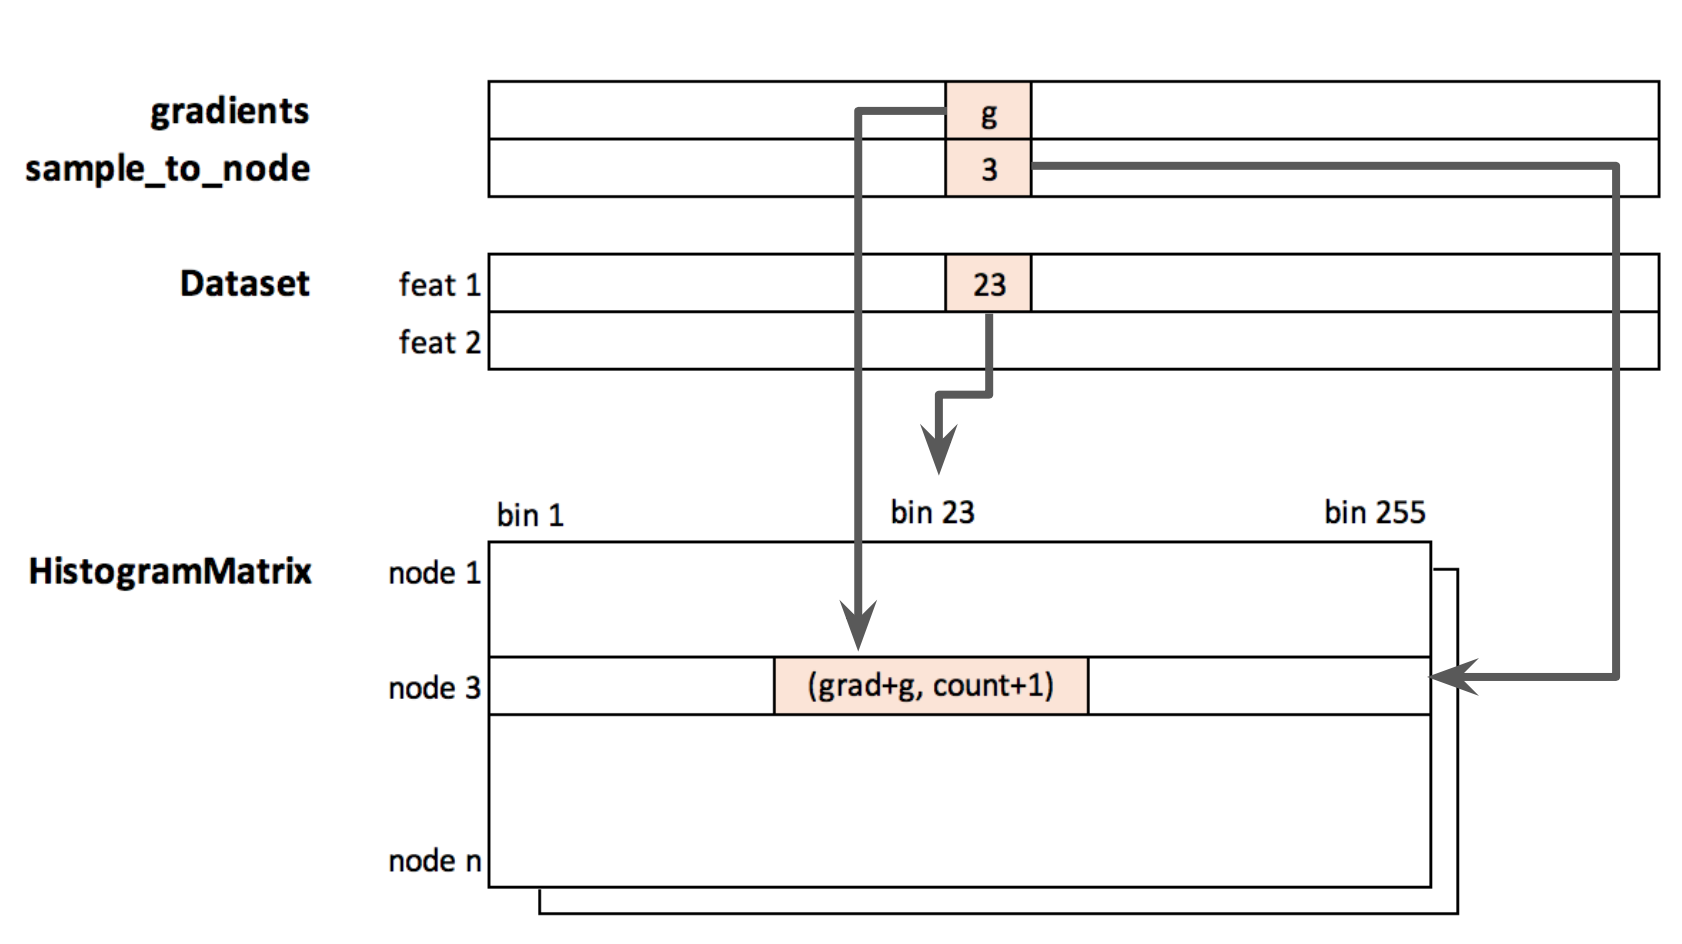
\includegraphics[width=0.47\textwidth]{fig/fig_v0.png}
  \caption{Illustration on updating a histogram bin.}
  \label{fig:baseline}
\end{figure}

Figure~\ref{fig:baseline} also illustrates the lack of locality in \update: \texttt{sample\_to\_node} and \texttt{feat} (a row in \texttt{Dataset}) represent the row and column index of a bin in \texttt{HistogramMatrix}, but both vectors are unordered. As a result, the accesses on \texttt{HistogramMatrix} are fully random, making it hard to parallelize or vectorize. Further, if we consider sorting either vector beforehand to improve locality, we will soon find that the accesses to \texttt{gradients} will become random. Since the size of \texttt{HistogramMatrix} is relatively small and fits into L3 cache, and the size of all other vectors are proportional to the number of samples, we believe it is the best choice to keep all other vectors sequentially accessed, at the cost of randomly accessing \texttt{HistogramMatrix}.

\mypar{\cumulate}
The bins are cumulated to transform the histogram into a suffix sum. After cumulating, each bin contains the sum of all bins starting from it until the last bin. This prepares the sums needed to calculate split gain in \getbestsplit.

\mypar{\getbestsplit}
To get the best split point of one histogram, we go over all bins to find the bin that gives the highest split gain. The right split gain is read directly from the cumulated histogram, while the left gain is calculated from the difference between the total and the right. To ensure no empty nodes are generated, the numbers of samples in both sides also needs to be checked.

\subsection{Feature Blocking}
In \findbestsplit, instead of processing one feature at a time, we block multiple features and process their histograms together.

\mypar{\update}
A crucial observation is that at line \ref{alg:split-grad}-\ref{alg:split-node} in Algorithm \ref{alg:split}, \texttt{gradients} and \texttt{sample\_to\_node} are same for all features of one data sample. 
Thus, we can reduce the accesses to these two vectors by feature blocking. As shown in Fig. \ref{fig:fb}, by processing multiple features at the same time, we can reduce the number of accesses to \texttt{gradients} and \texttt{sample\_to\_node} at the cost of maintaining a bigger HistogramMatrix. 


\begin{figure}[h]
  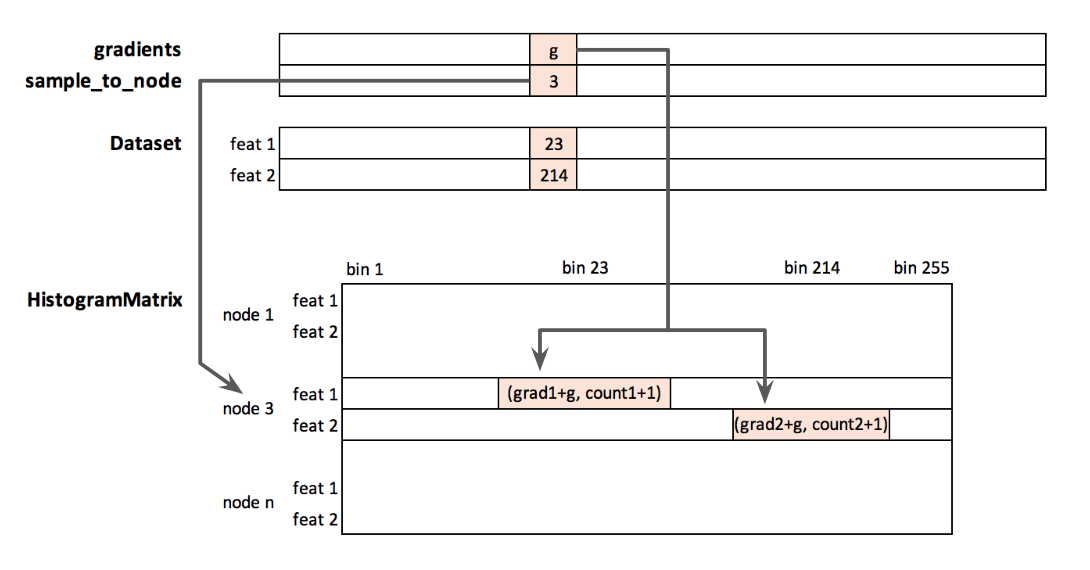
\includegraphics[width=0.47\textwidth]{fig/fig_fb.png}
  \caption{Illustration on feature blocking.}
  \label{fig:fb}
\end{figure}

\mypar{\cumulate}
To cumulate all the $sum\_count$ and $sum\_gradient$ in HistogramMatrix, we noticed that the summation always depends on the previous result and we can take advantage of instruction level parallelism by unrolling and introducing accumulators.
%Furthermore, we notice that there is no dependency across different even if there to increase the ILP
After feature blocking, we can further increase the number of accumulators on different features, and improve the \cumulate.

\mypar{\getbestsplit}
This function cannot directly benefit from feature blocking since the computation for splitGain of different thresholds are not dependent.

\subsection{Vectorization}
% Talk about transposed histogram later
We observed that it is hard to fully utilize the power of SIMD instructions in our case given the dependencies and our data format. 
% To circumvent those issues, we incorporate different strategies while optimizing each function individually. 

\mypar{\update}
\update cannot be vectorized directly as it follows a sequence of bin additions (RAW dependency) into the HistogramMatrix at indexes that cannot be calculated beforehand. Thus, if we vectorize consecutive additions into a single vectorized add, we would end up performing the incorrect operation. Additionally, if we need to perform update on the same bin, doing so would neglect the first three additions. To avoid this, we coupled additions with feature blocking to ensure that we write to different locations in our histogram matrix. 

As the update operations require access to bins at random locations, we make use of \texttt{gather} instructions from AVX-2. In order to use them, we treat addresses as raw integer values and calculate various offsets (using vector operations) to achieve our destination addresses, which are loaded using \texttt{gather}. After updating these values in-register, we store these values back into memory, one-by-one as \texttt{scatter} (store-equivalent of \texttt{gather}) is supported in AVX-512.

\mypar{\cumulate}
Notice that in \cumulate, the bin addition are performed in row major, and bins are added to the one next to them. That is, there are dependencies in every bin addition.
From this observation, it is hard to directly apply AVX vectorization, unless the histogram matrix is transposed and feature blocking is applied, so that the same bin of multiple features can be added at the same time. However, transposing the histogram could worsen the locality of \update as it turns the matrix to bin-major, but the variance of bins is higher than that of nodes. On the other hand, SSE vectorization can still be done since it only load/add one bin (two doubles), and thus avoids the dependency.

%In order to vectorize \cumulate directly, we would need to load bins at the same column but different (consecutive) rows, which introduces unnecessary overhead. To avoid this, we simply transpose our histogram matrix and thus, we need to load bins at same row but consecutive columns. However, since we need to store the results of addition back to memory at each step, we still incur significant overhead.

\mypar{\texttt{get\_best\_splits()}}
Similar to our previous argument, we need to compute values (square of gradients) along the bin-axis and thus, we can only vectorizing one bin (two doubles).
In order to perform vectorization, we combine \texttt{unpacklo/hi} to get a vector of gradinets and counts, and then use SIMD on the two doubles.

%this step would require us to transpose our histogram matrix to bin-major format. However, the \dots.

\subsection{Single-Precision Floating Point Computations}
For our data type optimization, we changed all instances of data type double to float. There are four main data structures that are affected by this change. They are the $scores$ and $gradients$ vectors, storing the sample scores and sample gradients respectively, the $thresholds$ vector that stores the threshold values for each bin, and the HistogramMatrix, which is of the type \texttt{vector\textless{vector}\textless{bin}\textgreater{}\textgreater{}} where bin contains two doubles.

By changing the data type from double to float, we reduced the amount of memory needed by one half. This also means theoretically we can fit twice as much data in each cache line using this optimization compared to our baseline implementation.

\mypar{\texttt{update()}}
From our perf profiling analysis, we found that our program incurs most of its cache misses around the additions of bin's $sum\_count$ and $sum\_gradient$, where the program increments $sum\_count$ by one, obtains the sample gradient from the gradient vector, adds to $sum\_gradient$, and stores both values back to the HistogramMatrix. While addition has the same latency for both doubles and floats, our program will benefit most from having less memory movement with the use of floats.

\mypar{\texttt{cumulate()}}
This function will not benefit much from using floats, because it contains only of sequential add operations of values within the HistogramMatrix.

\mypar{\texttt{get\_best\_splits()}}
This function contains multiple mul and div operations which will directly benefit from using a smaller datatype. In particular, division operation of floats has lower latency and higher throughput compared to that of doubles. Using floats should improve the performance of this function.

\subsection{Sparse Representation for Dataset}
It is a common pattern that the largest bin contains a great portion of samples. Therefore, we can transform the dataset into sparse representation, where every feature only stores the samples that do not fall into the largest bin. When doing histogram \update for a feature, a lot of samples will be skipped, and the information of the largest bin can be recovered by subtracting the sum of all other bins from the total statistics of the corresponding node, which has been stored in the node on its creation. 

This trick is one of the major optimizations in state-of-the-art libraries. However, this optimization reduces the running time by performing fewer flops instead of improving flop per cycle performance. The sparse representation is also hard to integrate with our other optimizations. As a result, we will only implement it and show the running time speedup, and will not include it in our further analysis.

\section{Experimental Results}\label{sec:exp}

\begin{figure*}[t!]
  \begin{minipage}{.45\textwidth}
      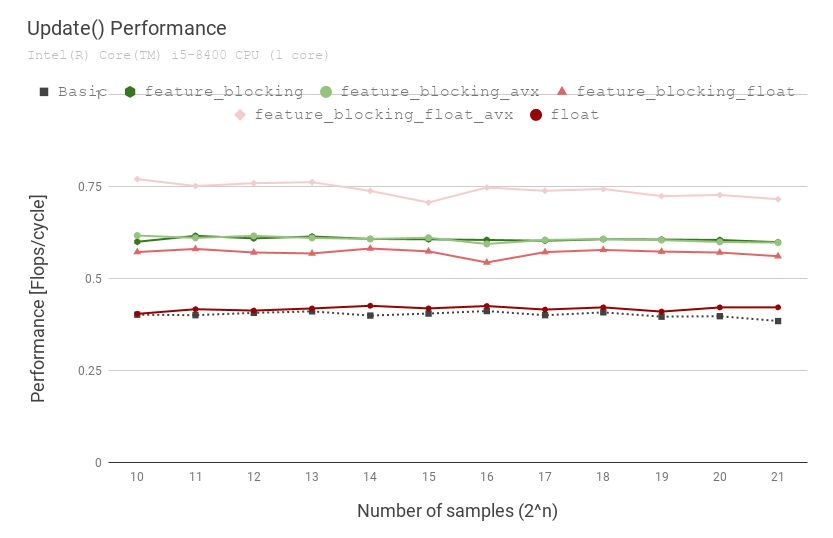
\includegraphics[width=1.0\textwidth]{fig/update.png}
      \caption{Performance of update().}
        \label{fig:update}
      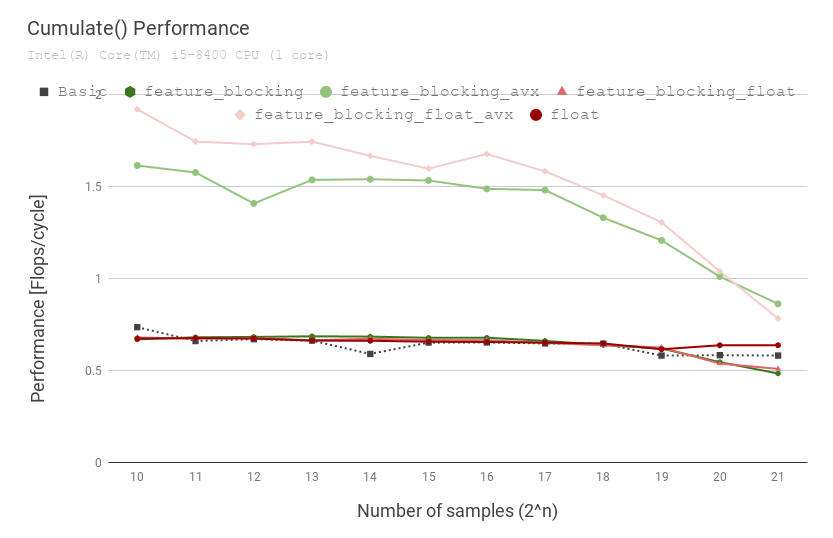
\includegraphics[width=1.0\textwidth]{fig/cumulate.png}
      \caption{Performance of cumulate().}
  \end{minipage} \quad \quad
  \begin{minipage}{.45\textwidth}
      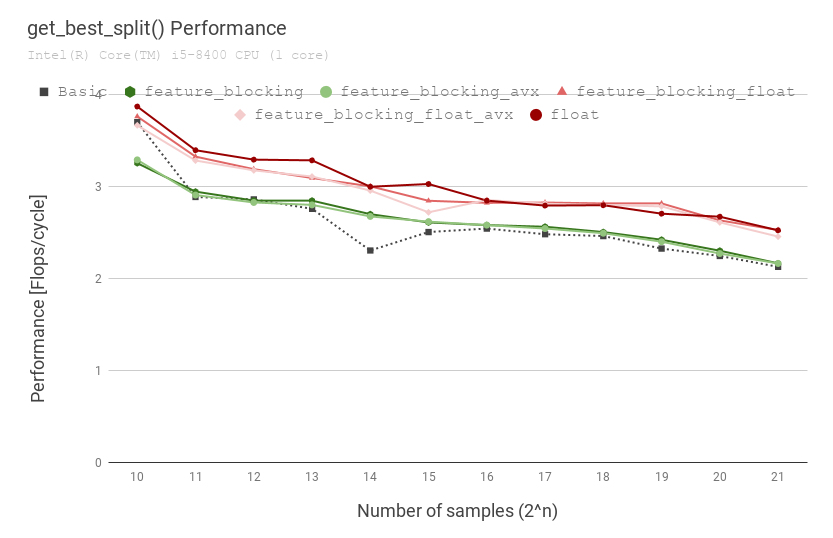
\includegraphics[width=1.0\textwidth]{fig/gbs.png}
      \caption{Performance of get\_best\_splits().}
      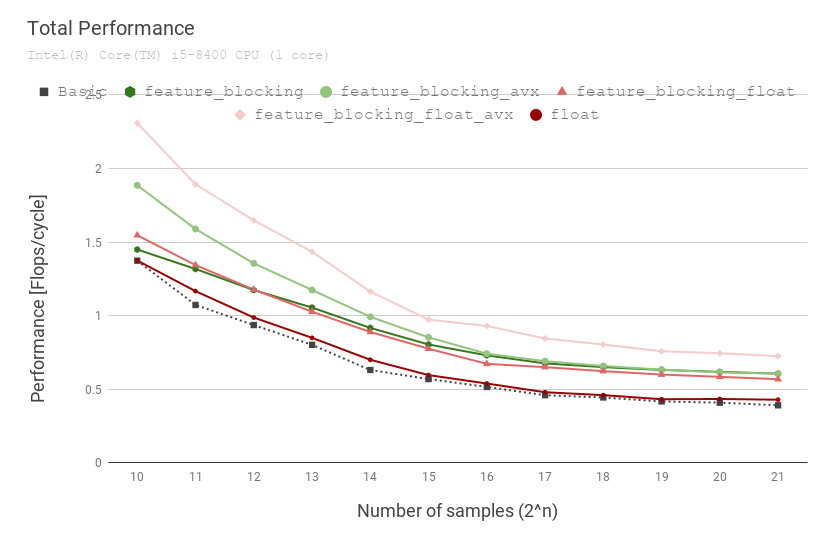
\includegraphics[width=1.0\textwidth]{fig/total.png}
      \caption{Performance of all three functions combined.}
        \label{fig:all}
  \end{minipage}
\end{figure*}
 
\mypar{Experimental setup} We ran our experiments on Intel(R) Core(TM) i5-8400 CPU @ 2.80GHz (Coffee Lake). The machine has L1 cache size of 32KB, L2 cache size of 256KB, and L3 cache size of 9216KB. Our experiments were run on Ubuntu 18.04 and compiled with gcc-7.3.0. We ran all our non-avx experiments with -O3 flag and avx experiments with -O3 -mfma -mavx flags.

We used the MSLR-WEB30K dataset from Microsoft Learning to Rank datasets\footnote{https://www.microsoft.com/en-us/research/project/mslr/}.
In order to compare the performance on different sizes of input, we cut the datasets to have sample numbers varying from $2^{10}$ to $2^{21}$. For each run, we set the number of trees to 10, maximum number of bins to 256, maximum depth to 9.


\mypar{Results}
Figures \ref{fig:update} to \ref{fig:all} show the experimental results of our proposed methods. The baseline method is always displayed in black, and the optimizations in different color gradients. We built our optimizations on top of each other to show that we combined the different optimizations to achieve the best program performance.

\mypar{\texttt{update()}}
The baseline performance of \texttt{update()} is around 0.4 flops/cycle. With our first feature blocking optimization, we were able to improve the performance to 0.6 flops/cycle. When we combined feature blocking with avx and single-precision floating point, the performance went up to 0.75 flops/cycle. For feature\_blocking\_float branch, we saw a significant performance gain going from no avx to avx, this is due to the fact that we are now loading, adding, and storing two single-precision floating points per cycle using packed-single instead of scalar-single instructions. For double-precision floating point branches (green lines in Figure 3), adding avx to our program allows us to load, add, and store two doubles in each cycle, and hence should increase our flop counts per cycle. On our Linux Coffee Lake machine, however, this change did not result in any improvements in performance. To further investigate this behavior, We ran these two branches on a Linux Haswell machine, and obtained a performance gain of 18 percent with the use of avx instructions. We proposed two possible explanations for this result. One possible explanation is that we cannot fully benefit from the performance of packed-double instructions since we are only vectorizing two doubles at a time. The more likely explanation is that our Coffee Lake machine might have done certain internal optimizations that improved the performance of scalar-double instructions, and thus our run resulted in a boosted performance.

The overall performance gain for this function is minimal due to the following reasons. First, for each \texttt{update()} call, we have both sequential and random accesses to the cache to load values into the registers. Then we perform two additions on the values, and store the updated values back to the cache. Although blocking was able to reduce the number of loads for the sequential accesses, it could not reduce the amount of random loads and stores, which occurs for sample size number of times per feature per depth per iteration. Second, we found through perf profiling that a large percentage of last level cache loads and misses occurred at loading in the bins to call \texttt{update()} on. The latency of the loads ended up dominating the runtime for each \texttt{update()} call. Third, we have an if statement before each \texttt{update()} call that determines whether or not the sample should be updated. This branching factor made any preloading or prefetching of the bins from the memory impossible.

\mypar{\texttt{cumulate()}}
Our plan to optimize \texttt{cumulate()} was to make use of blocking and instruction level parallelism. Since the bins of different nodes have no dependency on each other, we wanted to use accumulators in this function that would allow us to add the contents of the bins of multiple nodes at the same time. Our experimental result, however, shows that the non-avx version of this optimization did not improve the performance of the program in comparison to the baseline version (see dark green and dark pink lines in Figure 3). One of the reasons for this behavior is that when we loop through the bins to do the accumulation, we have to store the results back to the original bins in each round before we can proceed to the next. The lack of speedup is perhaps due to L1 cache store latency of around 4 cycles. To test our hypothesis, we removed the store instructions in this function and compared the difference in the number of cycles. We saw a 4x speedup in runtime, showing that the need to store values back to the bins in each round reduces the effectiveness of instruction level parallelism in this function. On the other hand, this function gets performance benefits from vectorization as we have expected. The light pink and light green lines in Figure 3 show that adding avx instructions and temporary variables to the function allows it to do two times more loads, adds, and stores per cycle, and to spend less time waiting on dependencies. Hence, we were able to get slightly more than 2x speedup.

\mypar{\texttt{get\_best\_split()}}
The only optimization done for this function is changing the datatype from double to float. As shown in Figure 4, we were able to get a 16 percent improvement in performance with this optimization. This is due mainly to the fact that floating point divisions of floats have lower latency than that of doubles.

\begin{figure}[h]
  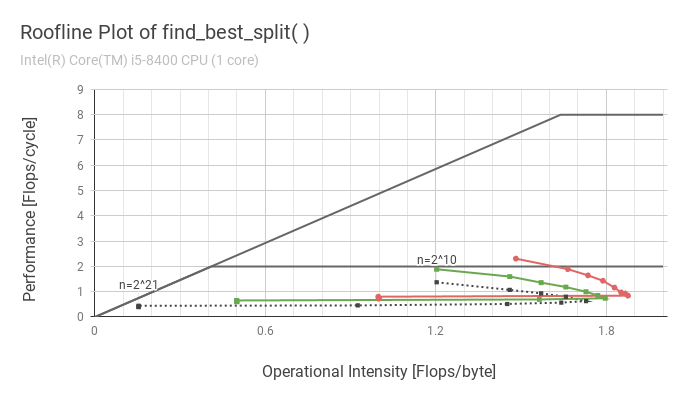
\includegraphics[width=0.47\textwidth]{fig/roofline.png}
  \caption{Roofline plot of various versions of find\_best\_split(). The baseline in black, feature\_blocking\_avx in green, feature\_blocking\_float\_avx in red.}
\end{figure}

\begin{figure}[ht]
  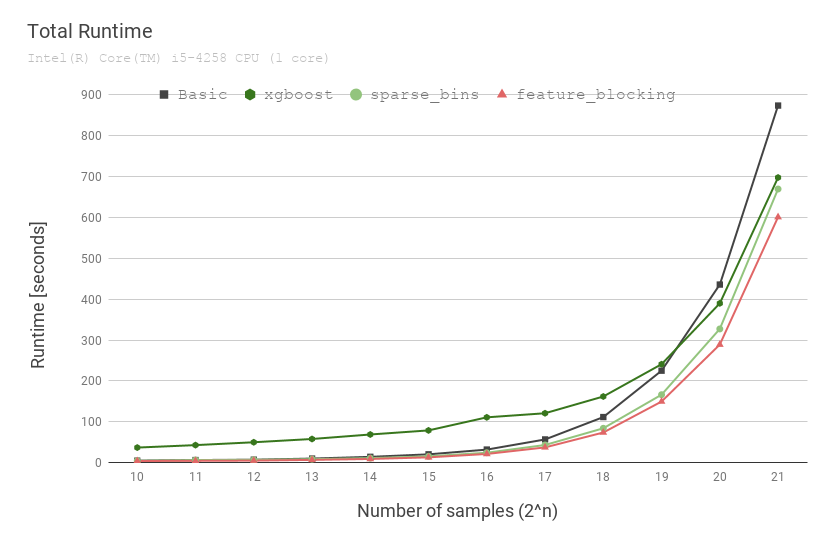
\includegraphics[width=0.47\textwidth]{fig/runtime.png}
  \caption{Runtime comparison of xgboost to our baseline, sparse bins, and feature blocking versions.}
\end{figure}

\section{Conclusions}
We began with a basic implementation of LambdaMART, a gradient boosting decision tree algorithm for learning to rank. From our basic implementation, we found the performance bottleneck of the program and identified the key function, \texttt{find\_best\_split()}. We then performed a few different versions of optimization on this function until we could get the most optimal performing version. We first added feature blocking and instruction level parallelism
%to the \texttt{update()} function within \texttt{find\_best\_split()}.
Then, we added AVX instructions to vectorize load, store and floating point add operations within the functions. Finally, we converted all occurrences of datatype double to float to speed up the performance even further. Overall, we obtained 1.93x speedup in \texttt{update()}, 2.6x speedup in \texttt{cumulate()} and 1.18x speed up in \texttt{get\_best\_split()}. Since \texttt{find\_best\_split()} is mostly dominated by the time spent on \texttt{update()}, in total we obtained a 1.7x speedup. 

We conclude the major challenges as (1) having relatively low arithmetic computations compared with extensive data loads and stores; (2) the working set is usually too large to be stored completely within caches; and (3) the operations are highly non-sequential and unpredictable thus making vectorization difficult.
%This is our very first attempt at optimizing a single-core gradient boosting decision tree algorithm. 
Although the speedup from the optimizations is not phenomenal, we were able to have an in-depth look and understanding of how this algorithm can be modified to work optimally in a single-core setting.

% References should be produced using the bibtex program from suitable
% BiBTeX files (here: bibl_conf). The IEEEbib.bst bibliography
% style file from IEEE produces unsorted bibliography list.
% -------------------------------------------------------------------------
\bibliographystyle{IEEEbib}
\bibliography{bibl_conf}

\clearpage
%\newpage
%\section*{Further comments [TO REMOVE]}

%Here we provide some further tips.

%\mypar{Further general guidelines}

%\begin{itemize}
%\item For short papers, to save space, I use paragraph titles instead of
%subsections, as shown in the introduction.

%\item It is generally a good idea to break sections into such smaller
%units for readability and since it helps you to (visually) structure the story.

%\item The above section titles should be adapted to more precisely
%reflect what you do.

%\item Each section should be started with a very
%short summary of what the reader can expect in this section. Nothing
%more awkward as when the story starts and one does not know what the
%direction is or the goal.

%\item Make sure you define every acronym you use, no matter how
%convinced you are the reader knows it.

%\item Always spell-check before you submit (to me in this case).

%\item Be picky. When writing a paper you should always strive for very
%high quality. Many people may read it and the quality makes a big difference.
%In this class, the quality is part of the grade.

%\item Books helping you to write better: {Higham:98} and {Strunk:00}.

%\item Conversion to pdf (latex users only): 

%dvips -o conference.ps -t letter -Ppdf -G0 conference.dvi

%and then

%ps2pdf conference.ps
%\end{itemize}

%\mypar{Graphics} For plots that are not images {\em never} generate (even as intermediate step)
%jpeg, gif, bmp, tif. Use eps, which means encapsulate postscript, os pdf. This way it is
%scalable since it is a vector graphic description of your graph. E.g.,
%from Matlab, you can export to eps or pdf.

%Here is an example of how to get a plot into latex
%(Fig.~\ref{fftperf}). Note that the text should not be any smaller than shown.

%\begin{figure}\centering
%  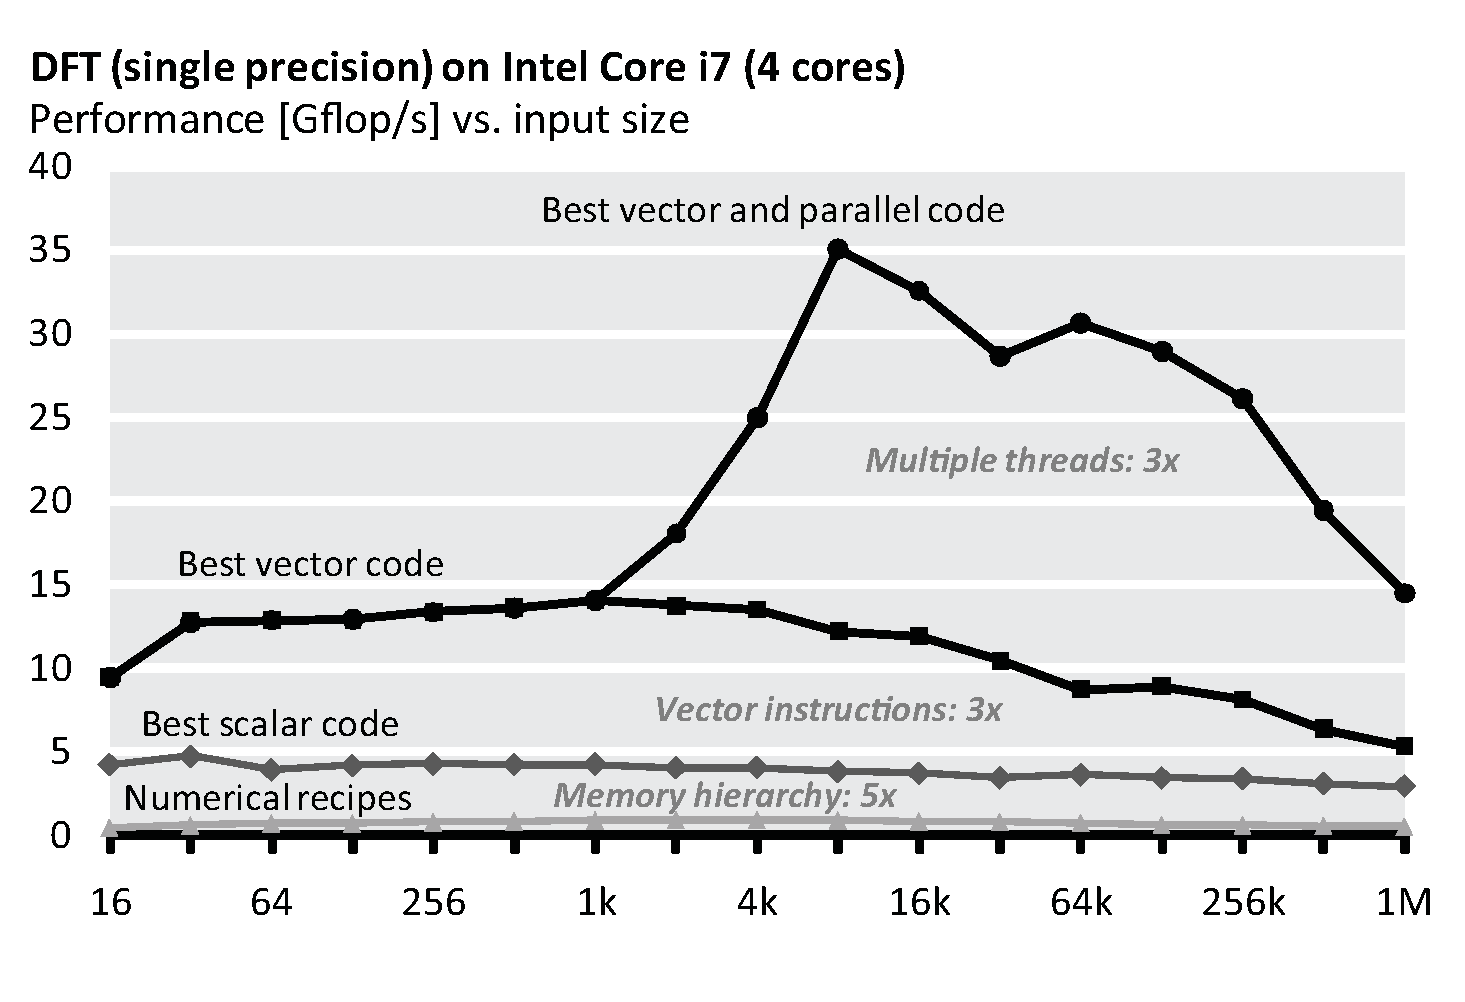
\includegraphics[scale=0.33]{dft-performance.eps}
%  \caption{Performance of four single precision implementations of the
%  discrete Fourier transform. The operations count is roughly the
%  same. {\em The labels in this plot are too small.}\label{fftperf}}
%\end{figure}

\end{document}

